% options:
% thesis=B bachelor's thesis
% thesis=M master's thesis
% czech thesis in Czech language
% slovak thesis in Slovak language
% english thesis in English language
% hidelinks remove colour boxes around hyperlinks

\documentclass[thesis=M,czech]{FITthesis}[2012/06/26]

\usepackage[utf8]{inputenc} % LaTeX source encoded as UTF-8

\usepackage{graphicx} %graphics files inclusion
% \usepackage{amsmath} %advanced maths
% \usepackage{amssymb} %additional math symbols

\usepackage{dirtree} %directory tree visualisation

\usepackage{nameref}
\usepackage{hyperref}
\usepackage{longtable}
\usepackage{pifont}

% % list of acronyms
% \usepackage[acronym,nonumberlist,toc,numberedsection=autolabel]{glossaries}
% \iflanguage{czech}{\renewcommand*{\acronymname}{Seznam pou{\v z}it{\' y}ch zkratek}}{}
% \makeglossaries

\newcommand{\tg}{\mathop{\mathrm{tg}}} %cesky tangens
\newcommand{\cotg}{\mathop{\mathrm{cotg}}} %cesky cotangens

% % % % % % % % % % % % % % % % % % % % % % % % % % % % % % 
% ODTUD DAL VSE ZMENTE
% % % % % % % % % % % % % % % % % % % % % % % % % % % % % % 

\department{Katedra softwarového inženýrství}
\title{Letecké záznamy pro iOS pomocí moderních architektur a FRP}
\authorGN{Martin} %(křestní) jméno (jména) autora
\authorFN{Žid} %příjmení autora
\authorWithDegrees{Bc. Martin Žid} %jméno autora včetně současných akademických titulů
\author{Martin Žid} %jméno autora bez akademických titulů
\supervisor{Ing. Dominik Veselý}

\acknowledgements{Doplňte, máte-li komu a za co děkovat. V~opačném případě úplně odstraňte tento příkaz.}

\abstractCS{
%TOTO NENI FINALNI VERZE
Tato práce realizuje iOS aplikaci pro evidenci letů.  V první části analyzuji obdobné aplikace a předpisy pro piloty České republiky, podle nichž probíhá návrh funkcionality vytvářené aplikace. Podle návrhu je následně zvolena vhodná architektura a vytvořeno uživatelského rozhraní v podobě wireframů.

Aplikace je implementována s použitím zvolené architektury a pomocí principů FRP. V průběhu implementace aplikace jsou realizovány jednotkové testy a na konci jsou provedeny uživatelské testy. Na základě výsledků testů je aplikace upravena do finální podoby.

V poslední části práce popisuji výhody a nevýhody, které přinesly postupy FRP. Také hodnotím časovou a implementační náročnost oproti standardním postupům a architektuře MVC. 

V~práci jsem vytvořil funkční iOS aplikaci s využitím moderní architektury a principů FRP. Aplikace bude sloužit pilotům České republiky pro elektronickou evidenci letů a bude jim také ulehčovat administrativu s evidencí spojenou.

V~příloze této diplomové práce je možné nalézt všechny zdrojové kódy jak aplikace, tak i testů společně s~vytvořenými wireframy.
}

\abstractEN{Sem doplňte ekvivalent abstraktu Vaší práce v~angličtině.}

\placeForDeclarationOfAuthenticity{V~Praze}
\declarationOfAuthenticityOption{4} %volba Prohlášení (číslo 1-6)
\keywordsCS{mobilní aplikace pro evidenci letů, iOS, Swift, FRP, ReactiveCocoa, MVVM architektura}
\keywordsEN{flight records mobile application, iOS, Swift, FRP, ReactiveCocoa, MVVM architecture}

\begin{document}

% \newacronym{CVUT}{{\v C}VUT}{{\v C}esk{\' e} vysok{\' e} u{\v c}en{\' i} technick{\' e} v Praze}
% \newacronym{FIT}{FIT}{Fakulta informa{\v c}n{\' i}ch technologi{\' i}}

\begin{introduction}
V dnešní době, kdy existují mobilní aplikace na téměř vše, mě zarazil fakt, že u pilotů tomu tak nemusí být. Aplikace na evidenci letů samozřejmě existují, však je tu hned několik problémů. Tyto aplikace jsou často velice drahé, nemusí odpovídat leteckým přepisům České republiky nebo nemají vyhovující funkcionalitu.

Z tohoto důvodu jsem se rozhodl vytvořit iOS aplikaci na evidenci letů. Tato aplikace bude pomáhat pilotům zaznamenávat elektronicky své lety, bude také kontrolovat předpisy a umožňovat export do formátu pro tisk.

Začínám analýzou podobných aplikací, a to pro zařízení iOS i Android. Poté navrhuji vhodnou funkcionalitu a vytvářím návrh uživatelského rozhraní.

Dalším tématem, které ve své práci řeším, jsou softwarové architektury při vývoji iOS aplikace. Zde analyzuji alternativy k architektuře MVC ve spojení s funkcionálně reaktivním programováním neboli FRP.

Tuto analýzu následně aplikuji v praxi, kdy se zvolenou architekturou a FRP implementuji společně s jednotkovými testy dříve zmíněnou aplikaci. Nakonec aplikaci podrobím uživatelským testům a podle jejich výsledků
upravím aplikaci do finální podoby.

V poslední části své práce se snažím zhodnotit postupy FRP společně se mnou zvolenou moderní architekturou a jejich časovou a implementační náročnost oproti klasickému MVC.
\end{introduction}

\chapter{Cíl práce}
Cílem této práce je navrhnout a implementovat aplikaci k evidenci letů pro platformu iOS, a to pomocí postupů FRP (funkcionálně reaktivního programování) a s využitím moderní softwarové architektury jako např. MVVM nebo VIPER.  Tato aplikace bude sloužit pilotům České republiky k elektronické evidenci letů. Tento cíl je rozdělen do několika podúkolů.

V první části analyzuji podobné aplikace pro evidenci letů, a to jak pro platformu iOS, tak i pro Android. Na základě této analýzy navrhnu vhodnou funkcionalitu pro vytvářenou aplikaci. Podle navržených funkcionalit si zvolím architekturu  a navrhnu uživatelské rozhraní v podobě wireframů.

V dalším kroku aplikaci implementuji pomocí postupů FRP a se zvolenou architekturou. V průběhu realizace aplikace budou vytvářeny také testy a dokumentace aplikace.

Dále bude aplikace podrobena uživatelským testům, podle kterých bude vhodně upravena.

V poslední části budu popisovat výhody a nevýhody, které přinesly postupy FRP. Budu také hodnotit časovou a implementační náročnost oproti standardním postupům a architektuře MVC. 


\chapter{Analýza a návrh}

\section{Tvorba iOS aplikací}
Vývoj iOS aplikace je možný hned několika způsoby, každý má své výhody a nevýhody, právě ty bych rád v této kapitole rozebral. Mezi možné způsoby vývoje bych rád zmínil nativní aplikace, hybridní aplikace a mobilní webové aplikace.

\subsection{Nativní aplikace}
Nativní aplikace jsou vyvíjeny specificky pro jednu platformu. Díky tomu mají přístup ke všem funkcím daného zařízení jako např. GPS, kamera nebo kontakty. Mohou fungovat i pouze offline, tedy bez nutnosti internetového připojení. \cite{Nielsen}

Však pokud bychom chtěli aplikaci distribuovat na více platforem, tak s tímto přístup by bylo nutné vytvořit pro každou platformu vlastní aplikaci. To by prodloužilo vývoj a znesnadnilo následnou údržbu aplikací.

Co se týče iOS vývoje, je možné si zvolit z dvou programovacích jazyků -- Objective-C nebo Swift. \cite{objc} \cite{swift}

\subsection{Hybridní aplikace}
Hybridní aplikace jsou aplikace tvořené nejčastěji pomocí HTML5 a JavaScriptu, následně jsou spuštěné v nativním kontejneru. \cite{saleforce} Jako příklad je možné uvést např. Apache Cordova. Tento kontejner umožňuje přístup k funkcím daného přístroje, podporuje použití aplikace offline a dává možnost publikace vytvořené aplikace do obchodu tzv. app store. \cite{cordova}

Však výhodou nativních aplikacím proti hybridním je to, že jsou vytvářeny přesně pro danou platformu, a tudíž jejich vzhled a výkon bude vždy lepší. \cite{upwork}

\subsection{Mobilní webové aplikace}
Poslední možností jsou mobilní webové aplikace. Tyto aplikace jsou pouze upravené webové stránky do podoby a chování nativních aplikací. Přestože běží pouze v prohlížeči, mohou mít i tyto aplikace přístup k určitým (ne však ke všem) nativním funkcím. \cite{Nielsen}

Tím, že jsou mobilní webové aplikace spouštěny v prohlížeči a nejsou stahovány přes obchody, je ulehčena údržba a vývoj, protože si uživatel nemusí vždy stahovat novou verzi aplikace.

Však tento postup má i své nevýhody. Jak již bylo zmíněno dříve, aplikace nemá přístup ke všem nativním funkcím daného přístroje. S dalším problémem se můžeme setkat u offline ukládání dat, a to se zabezpečením, které nemusí být tak dokonalé nebo uživatelsky přívětivé, jako u nativních aplikací.  \cite{saleforce}

\subsection{Zvolené řešení}
Pro svou práci jsem si zvolil možnost nativní mobilní aplikace z důvodu zaměření pouze na platformu iOS. Bude se tedy jednat pouze o jednu aplikaci, která bude moci využít všech nativních funkcionalit, výkonu i vzhledu.

\section{EASA}
EASA, neboli European Aviation Safety Agency, je agentura spadající pod Evropskou Unii, která má na starosti technické přepisy, bezpečnost, regulace a certifikace v oboru letectví. \cite{EU} 

Pro tuto diplomovou práci je EASA důležitá, protože vydává i pokyny např. pro evidenci letů nebo limity odlétaných hodin. \cite{EASARegulations}

\subsection{Pokyny pro evidenci letů}
Pokyny pro evidenci letů udává předpis FCL.050. Tento předpis specifikuje povinné položky každého leteckého záznamu. \cite{FCL} 

\uv{
Každý záznam letů by měl obsahovat minimálně tyto informace:
\begin{enumerate}
\item osobní informace: jméno a adresu pilota;
\item každý záznam letu by měl obsahovat:
	\begin{itemize}
	\item jméno velícího pilota (PIC -- Pilot-in-command),
	\item datum letu,
	\item čas a místo odletu a příletu,
	\item typ, značku, model, variantu a registraci letadla,
	\item označení zda je letadlo jednomotorové (SE -- single engine) nebo vícemotorové (ME -- multi engine),
	\item čas letu,
	\item celkový čas letu.
	\end{itemize}
\item každý záznam z výcvikového zařízení pro simulaci letu (FSTD -- flight simulation training devices) by měl obsahovat:
	\begin{itemize}
	\item typ a kvalifikační číslo výcvikového zařízení,
	\item instrukce výcvikového zařízení pro simulaci letu,
	\item datum,
	\item čas,
	\item celkový čas.
	\end{itemize}
\item funkce pilota -- velící pilot (včetně sólového, velícím pilotem student (Student PIC) nebo velící pilot pod dohledem (PICUS -- pilot-in-command under supervision)), druhý pilot, dvojí pilot (dual), instruktor (FI -- Flight Instructor) nebo zkoušející (FE -- Flight Examiner);
\item provozní podmínky -- pokud se let uskutečnil v noci nebo pokud byl prováděn podle pravidel pro let podle přístrojů.
\end{enumerate}
} \cite{FCL} (překlad vlastní)

\subsection{Limity}
Limity letového času a času ve službě obsahuje předpis ORO.FTL.210.

\uv{
Celková doba služby, na kterou může být člen posádky přidělen, nesmí překročit:
\begin{enumerate}
\item 60 hodin služby za 7 po sobě jdoucích dnů;
\item 110 hodin služby za 14 po sobě jdoucích dnů; a 
\item 190 hodin služby za 28 po sobě jdoucích dnů, rozdělených co nejrovnoměrněji během tohoto období.
\end{enumerate}
Celkový čas, na který je jedinec přidělen jako člen provozní posádky, nesmí překročit:
\begin{enumerate}
\item 100 hodin letu za 28 po sobě jdoucích dnů;
\item 900 hodin letu v kalendářním roce; a
\item 1000 hodin letu během 12 po sobě jdoucích kalendářních měsících.
\end{enumerate}
Poletová služba se počítá do doby služby.
} \cite{FTL} (překlad vlastní)

\subsection{Zdravotní certifikáty}
Informace o zdravotních certifikátech obsahuje předpis Part-MED. Certifikáty jsou tří druhů -- zdravotní certifikát třídy 1 (Class 1 medical certificate), zdravotní certifikát třídy 2 (Class 2 medical certificate) a zdravotní certifikát pro licence na lehká letadla (LAPL -- Light Aircraft Pilot Licence). Každý z těchto certifikátů má jinak nastavenou dobu platnosti a je pro jiné typy pilotních licencí.

LAPL certifikát je pouze pro pilotní licence na lehká letadla. Platnost je 60 měsíců u pilotů do věku 40 let, poté je platnost pouze 24 měsíců.

Zdravotní certifikát třídy 2 je pro pilotní licence PPL (Private Pilot Licence), SPL (Sailplane Pilot Licence) a BPL (Balloon Pilot Licence), tedy pro piloty soukromých letadel, kluzáků a balónů. Platnost licence se znovu odvíjí od věku pilota -- 60 měsíců u pilotů do věku 40 let, následně 24 měsíců do věku 50 let a nakonec platnost licence klesá na 12 měsíců.

Zdravotní certifikát třídy 1 je certifikát nejvyšší úrovně. Je pro pilotní licence CPL (Commercial Pilot Licence), MPL (Multi-crew Pilot Licence) a ATPL (Airline Transport Pilot Licence), tedy pro piloty komerčních, vícečlenných a dopravních letadel. Platnost licence je 12 měsíců. To neplatí u pilotů starších 40 let, létajících jednopilotní komerční lety s cestujícími nebo u pilotů starších 60 let, zde se platnost licence snižuje na 6 měsíců. \cite{CAA}

\section{Analýza existujících aplikací pro evidenci letů}
Tato kapitola se zabývá analýzou již existujících aplikací pro evidenci letů. Pro analýzu bylo vybráno pět aplikací -- tři pro iOS a dvě pro platformu Android.
\begin{enumerate}
\item LogTen Pro X -- iOS aplikace v angličtině vyvíjená společností Coradine Aviation. \cite{appStoreLogTen}
\item Logbook Pro Aviation Flight Log for Pilots -- druhá iOS aplikace, také v angličtině, vytvořená NC Software, Inc. \cite{appStoreLogbookPro}
\item Safelog Pilot Logbook -- poslední z analyzovaných iOS aplikací. I tato aplikace je v anglickém jazyce. Publikována Dauntless Software. \cite{appStoreSafeLog}
\item FlyLogio - Pilot Logbook -- česká aplikace vyvinutá pro platformu Android společností FlyLogio.com. \cite{googleFlyLogio}
\item Smart Logbook -- anglická Andriod aplikace vydána firmou Kviation, Inc. \cite{googleSmartLogbook}
\end{enumerate}

\begin{figure}[]\centering
 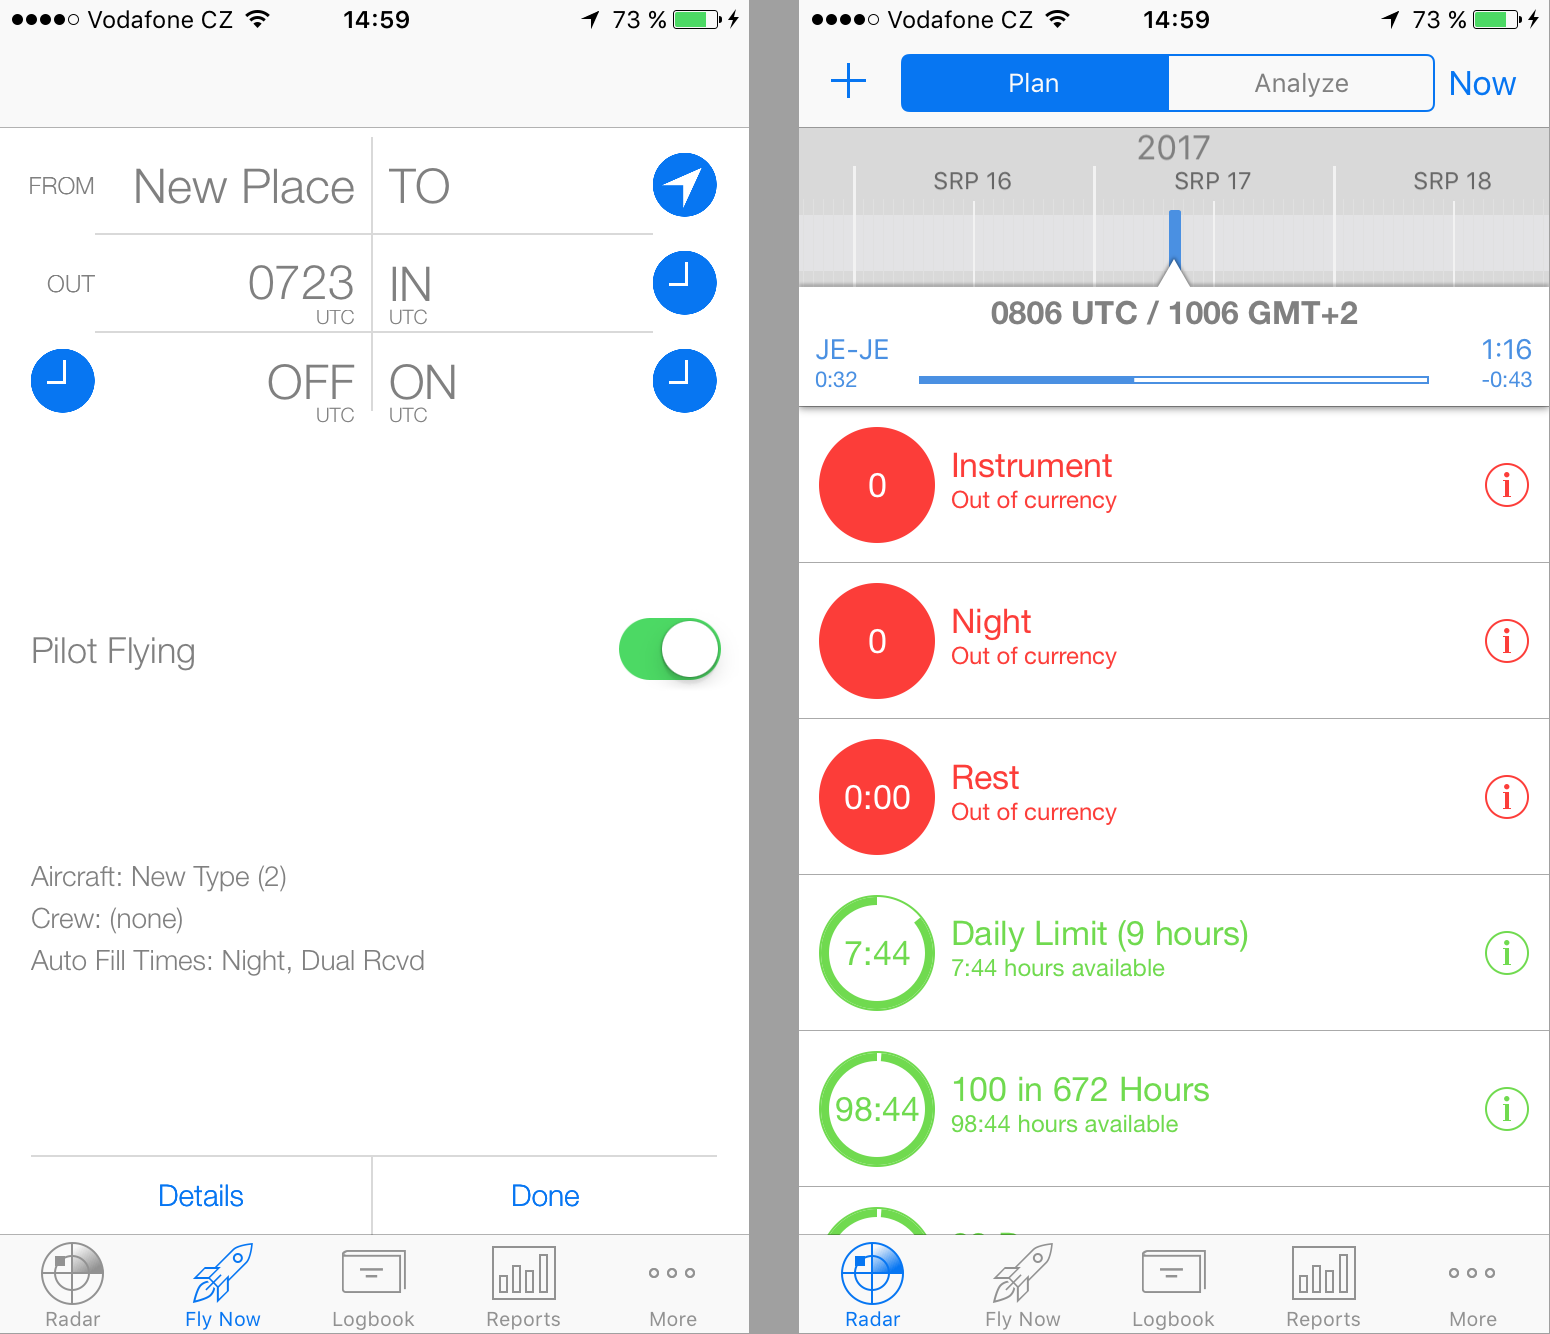
\includegraphics[width=0.99\textwidth]{./pictures/existujiciAplikace/LogTenProX}
 \caption[LogTen Pro X]{LogTen Pro X}\label{fig:LogTenProX}
\end{figure}

\begin{figure}[]\centering
 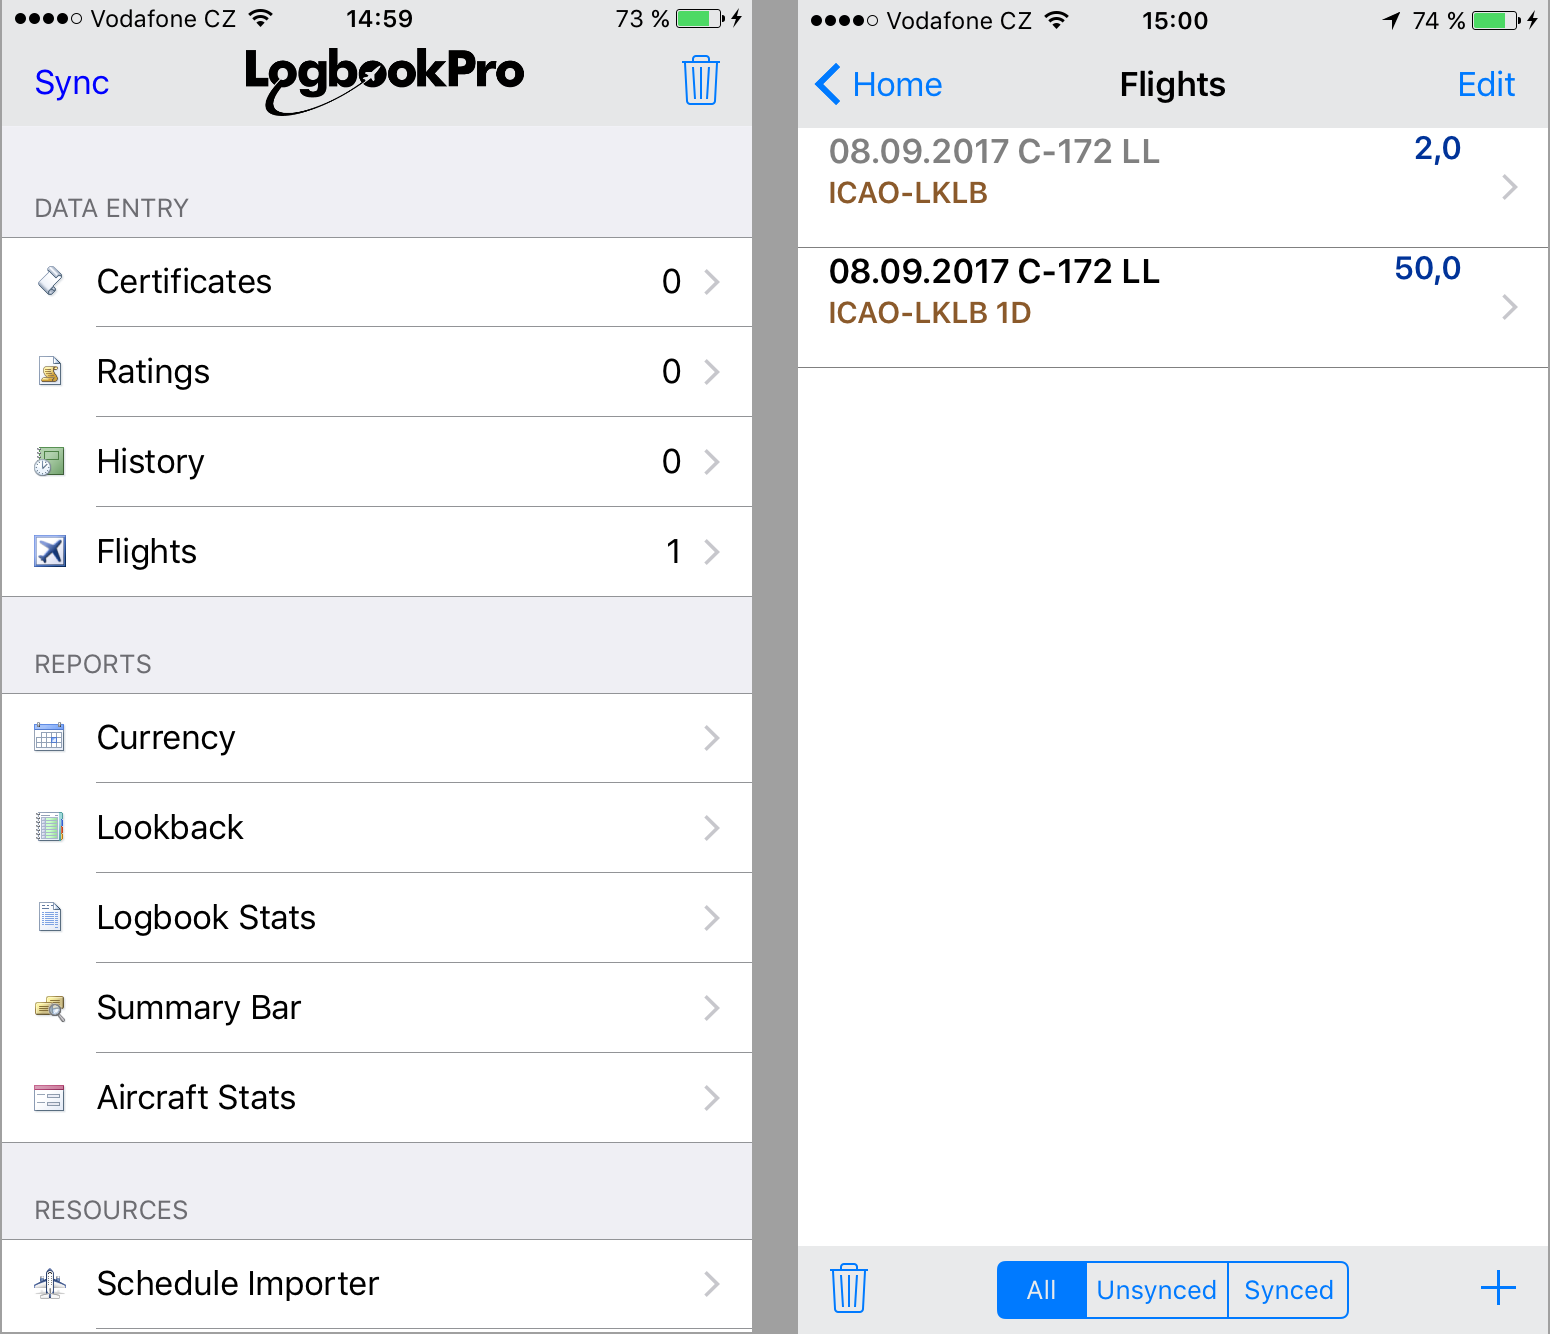
\includegraphics[width=0.99\textwidth]{./pictures/existujiciAplikace/LogbookPro}
 \caption[Logbook Pro Aviation Flight Log for Pilots]{Logbook Pro Aviation Flight Log for Pilots}\label{fig:LogbookPro}
\end{figure}

\begin{figure}[]\centering
 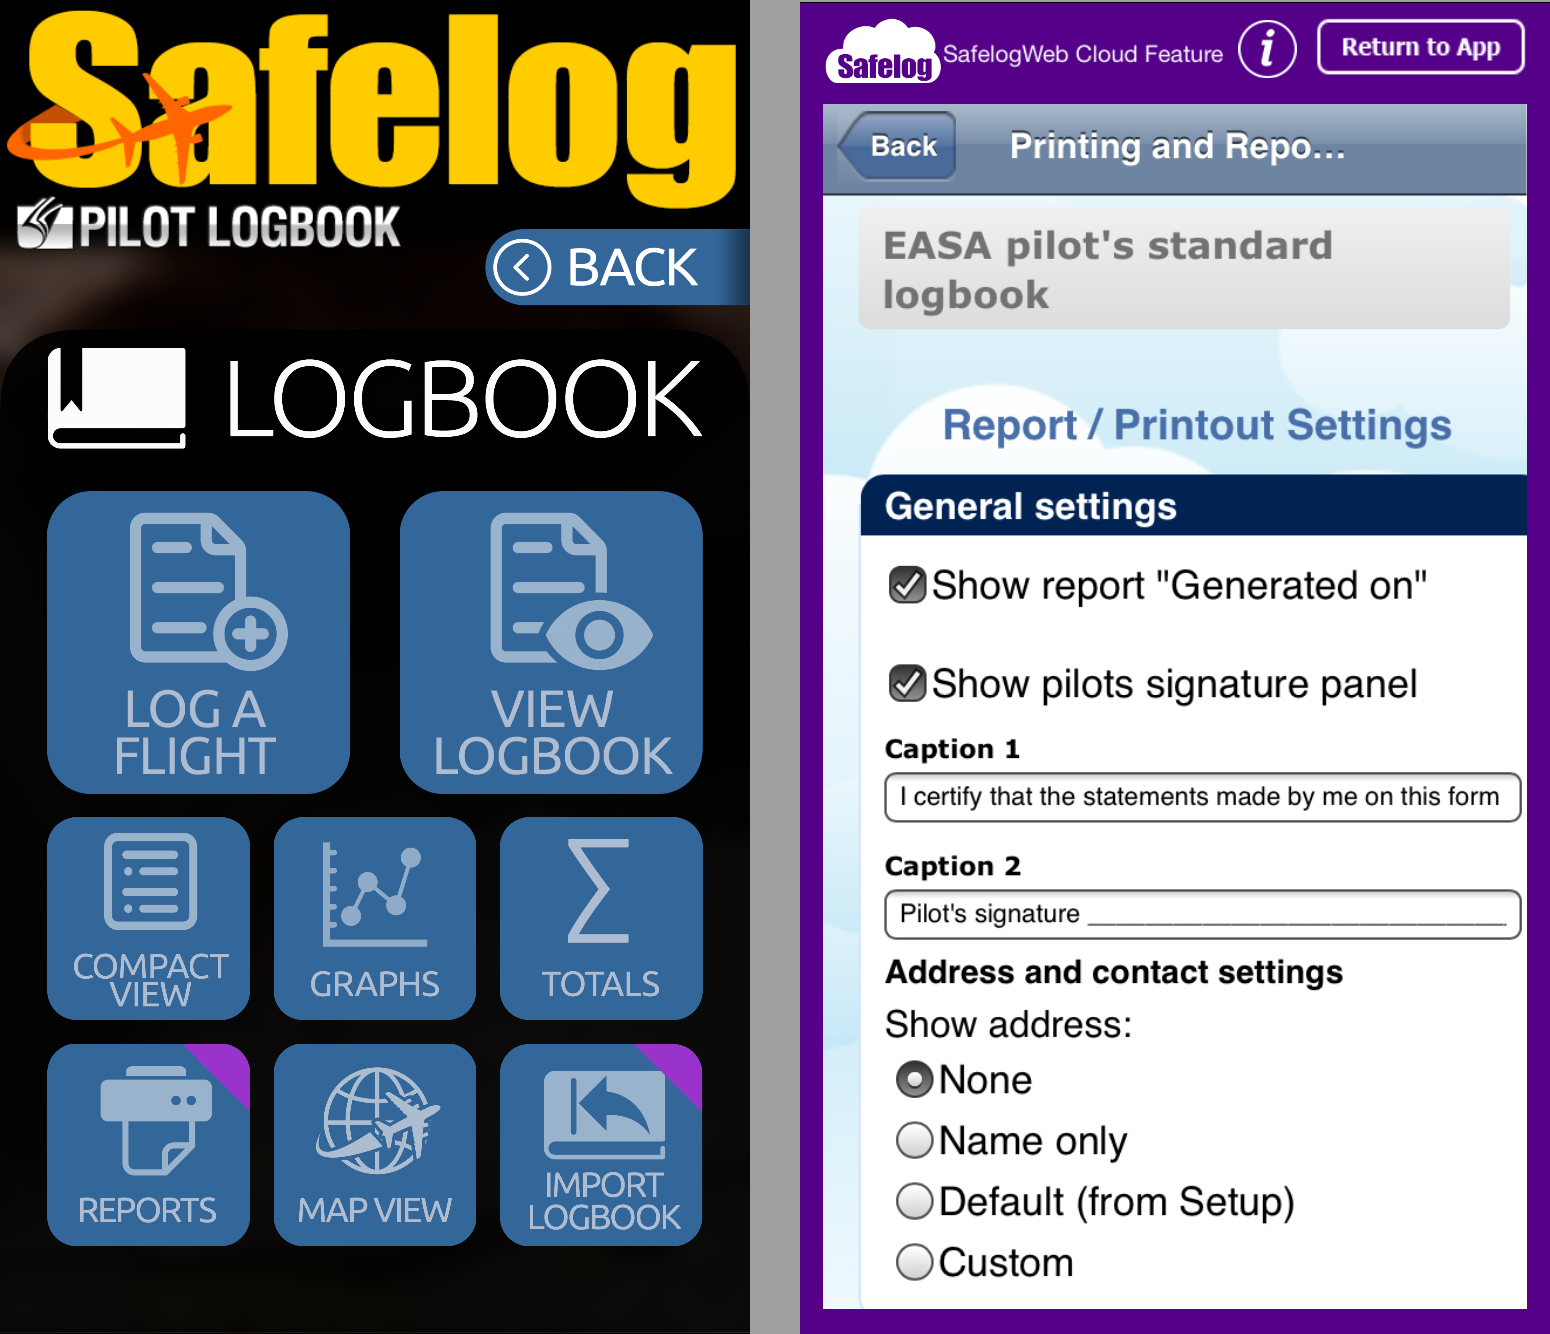
\includegraphics[width=0.99\textwidth]{./pictures/existujiciAplikace/Safelog}
 \caption[Safelog Pilot Logbook ]{Safelog Pilot Logbook }\label{fig:Safelog}
\end{figure}

\begin{figure}[]\centering
 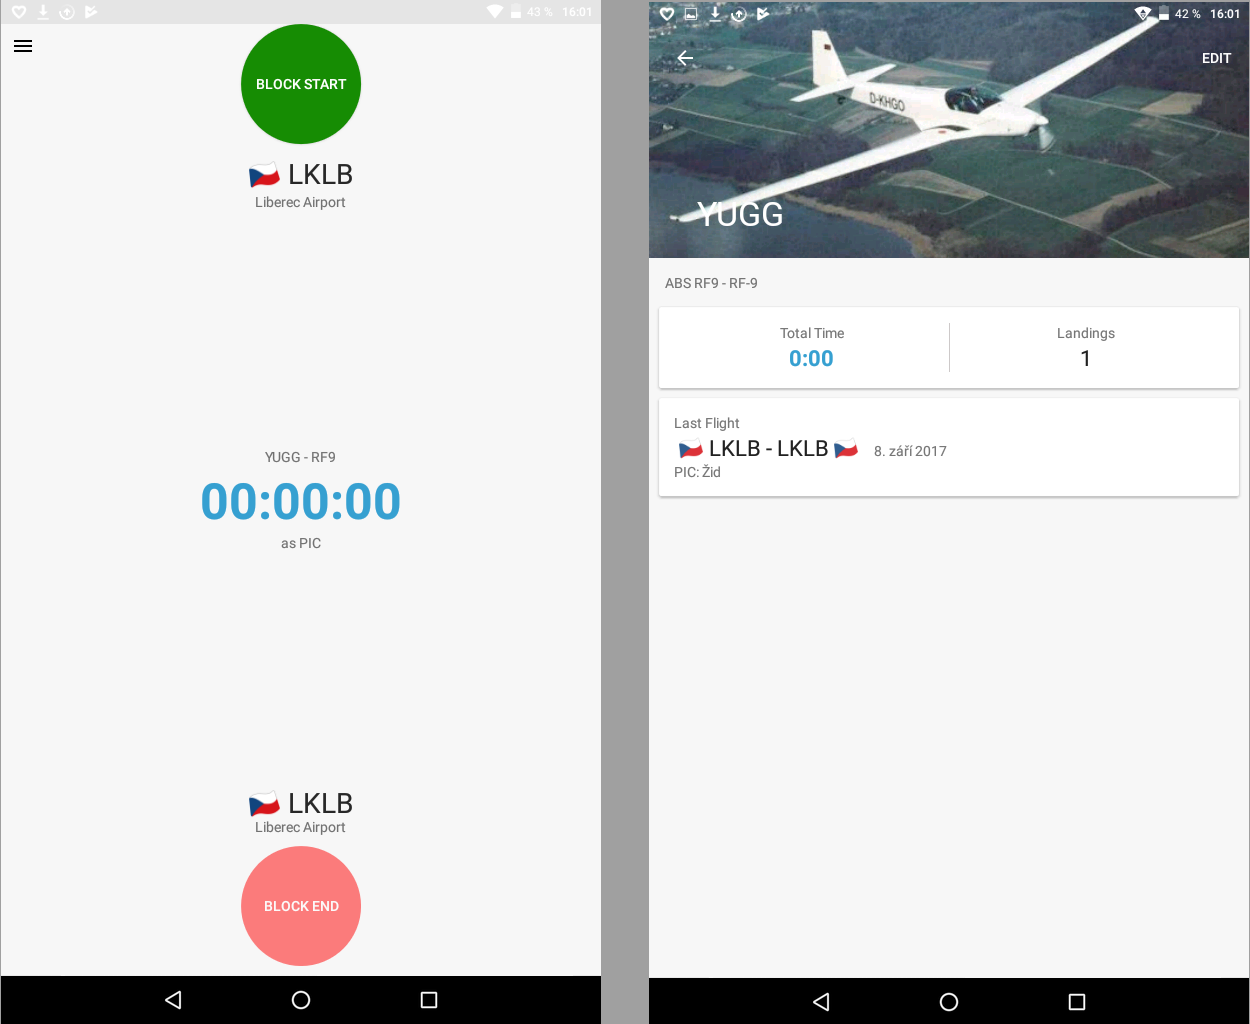
\includegraphics[width=0.99\textwidth]{./pictures/existujiciAplikace/FlyLogio}
 \caption[FlyLogio]{FlyLogio}\label{fig:FlyLogio}
\end{figure}

\begin{figure}[]\centering
 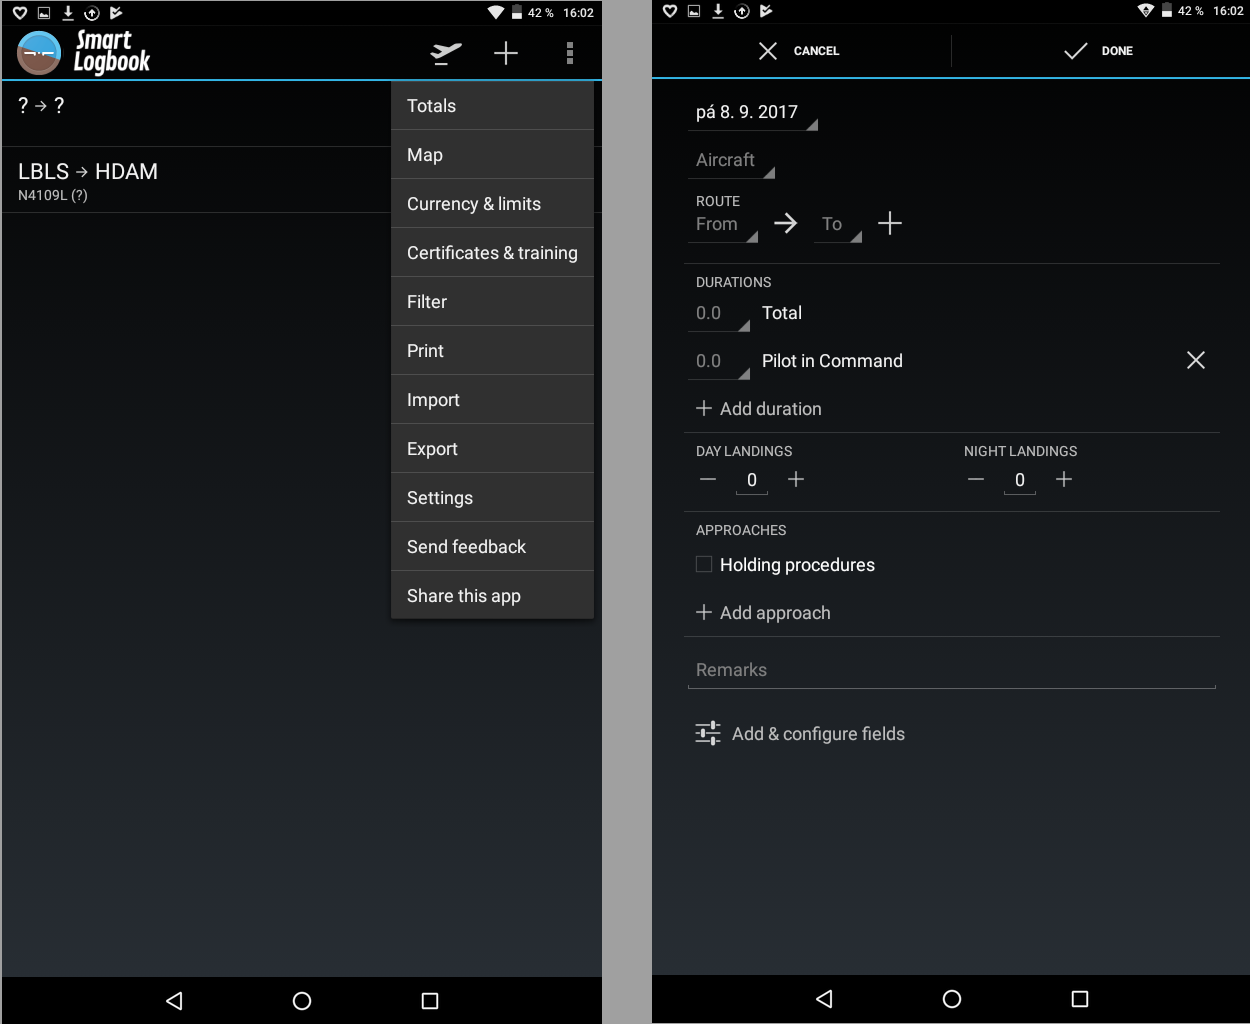
\includegraphics[width=0.99\textwidth]{./pictures/existujiciAplikace/SmartLogbook}
 \caption[Smart Logbook]{Smart Logbook}\label{fig:LogTenProX}
\end{figure}

\subsection{Kritéria hodnocení}
Kritéria hodnocení byla rozdělena do několika kategorií -- přihlášení, platby, napojení externích databází, doplňkové položky při vkládání záznamu, limity a certifikáty, reporty a zálohování.	

Při vkládání záznamu jsou brány v potaz pouze doplňkové položky, protože aplikace bude tvořena podle předpisu EASA FCL.050, který udává povinné údaje při evidování letu. Také položka v hodnocení  -- reporty podle EASA, je analyzována z pohledu předpisu FCL.050. 

Všechny položky hodnocení jsou uváděny z pohledu mobilní/tablet aplikace.

\subsection{Srovnávací tabulka}
\newcommand{\OK}{\ding{51}}
\newcommand{\NOK}{\ding{55}}
\newcommand{\rot}{\rotatebox{90}}

{\setlength\extrarowheight{2pt}
\begin{longtable}{@{\extracolsep{\fill}}l c c c c c c}
   \caption[Srovnávací tabulka]{Srovnávací tabulka}\label{tab:srovnavaci_tabulka} \\
   Kritéria & \rot{Log Ten Pro X} & \rot{Logbook Pro} & \rot{Safelog} &
   \rot{FlyLogio} & \rot{Smart Logbook} & \rot{Výsledek} \\
  \endfirsthead
   \caption[Srovnávací tabulka]{Srovnávací tabulka}\label{tab:srovnavaci_tabulka} \\
   Kritéria & \rot{Log Ten Pro X} & \rot{Logbook Pro} & \rot{Safelog} &
   \rot{FlyLogio} & \rot{Smart Logbook} & \rot{Výsledek} \\
  \endhead

   \hline
   \multicolumn{7}{c}{Přihlášení} \\
   \hline
   Aplikace funkční bez přihlášení 			 & \OK & \NOK & \NOK & \NOK & \NOK & 1/5 \\
   Možnost přihlášení								 & \OK & \OK & \OK & \OK & \OK  & 5/5 \\
   
   \hline
   \multicolumn{7}{c}{Platby} \\
   \hline
   Platby jednorázové			 & \NOK & \NOK & \NOK & \NOK & \OK & 1/5 \\
   Opakované platby			 & \OK & \OK & \OK & \OK & \OK  & 5/5 \\
   
   \hline
   \multicolumn{7}{c}{Napojení externích databází} \\
   \hline
   Napojení na databázi letišť		 & \NOK & \OK \footnote{Logbook Pro umí nalézt pouze nejbližší letiště.} & \OK & \OK & \OK & 4/5 \\
   Napojení na databázi letadel	 & \NOK & \NOK & \OK & \OK & \NOK  & 2/5 \\
   
   \hline
   \multicolumn{7}{c}{Doplňkové položky při vkládání záznamu} \\
   \hline
   Možnost přidání fotky						 & \OK & \NOK & \OK & \NOK & \NOK & 2/5 \\
   Možnost přidání dokumentu			 & \OK & \NOK & \OK & \NOK & \NOK & 2/5 \\
   
   \hline
   \multicolumn{7}{c}{Limity a certifikáty} \\
   \hline
   Kontrola limitů					 & \OK & \OK & \OK \footnote{Safelog zobrazuje limity ve webové verzi.} & \NOK & \OK & 4/5 \\
   Certifikáty							 & \OK & \OK & \OK \footnote{Safelog zobrazuje certifikáty ve webové verzi.} & \NOK & \OK & 4/5 \\
   
   \hline
   \multicolumn{7}{c}{Reporty} \\
   \hline
   Generování reportů					 & \OK & \NOK & \OK \footnote{Safelog zobrazuje reporty ve webové verzi.}  & \NOK & \OK & 3/5 \\
   Reporty podle EASA					 & \NOK & \NOK & \OK & \NOK & \OK & 2/5 \\
   Jiné reporty								 & \OK & \OK & \OK & \NOK & \OK & 2/5 \\
   
   \hline
   \multicolumn{7}{c}{Perzistence dat} \\
   \hline
   iCloud/Google					 & \OK & \NOK & \NOK & \OK & \OK & 3/5 \\
   Vlastní řešení						 & \NOK & \OK & \OK & \NOK & \NOK & 2/5 \\
   Synchronizace více zařízení  & \OK & \OK & \OK & \OK & \OK & 5/5 \\

\end{longtable}
}
\subsection{Výsledky a vlastní zhodnocení}
\subsubsection{LogTen Pro X}
LogTen Pro X je z analyzovaných iOS aplikací nejvíce uživatelsky přívětivá. Zobrazuje přehledně limity a certifikáty, i vkládání je intuitivní. Má však i několik nedostatků: 
\begin{itemize}
\item není napojená na databázi letišť, tudíž uživatel musí vyplnit všechny informace o daném letišti sám, bez automatického doplnění nebo našeptávání;
\item neumožňuje generování reportů podle předpisu EASA FCL.050;
\item aplikace je placená ročně --
	\begin{itemize}
	\item iPhone + iPad + Mac -- 3550 Kč,
	\item Mac -- 3550 Kč,
	\item iPhone + iPad -- 2150 Kč.
	\end{itemize}
\end{itemize}
Data o aplikaci a cenách jsou získány přímo z aplikace LogTen Pro X. 

\subsubsection{Logbook Pro Aviation Flight Log for Pilots}
Aplikace Logbook Pro vyžaduje pro přihlášení stažení PC aplikace (pouze pro Windows). S touto aplikací je následně synchronizován. Některá funkcionalita, např. generování reportů, je dostupná pouze v PC verzi.

PC verze aplikace je zadarmo pouze ve zkušební verzi, poté základní verze stojí v přepočtu 1800 Kč. iOS verze aplikace se platí ročně v přepočtu za 1045 Kč, je nutné si zaplatit i zálohování a další funkcionality. \cite{SafelogPrices}

\subsubsection{Safelog Pilot Logbook}
Safelog Pilot Logbook obsahuje pouze některé funkce přímo v aplikaci, u ostatních je uživatel odkázán do webového rozhraní (SafelogWeb Cloud) viz. \ref{fig:Safelog}. Toto webové rozhraní zobrazené v aplikaci však není přizpůsobené pro mobilní zařízení, často je zobrazena pouze část stránky a není možné např. vyplnit všechna pole formuláře.

Tato aplikace však, pokud budeme brát v potaz i funkce ve webovém rozhraní, obsahuje nejširší spektrum funkcionalit.

Samotná aplikace je zadarmo, ale pro plnou verzi aplikace je nutné předplatné. To se pohybuje od 1320 Kč za jeden rok až po 8990 Kč za deset let. Data o aplikaci a cenách jsou získány z aplikace Safelog Pilot Logbook.

\subsubsection{FlyLogio - Pilot Logbook}
Android aplikace FlyLogio - Pilot Logbook je jedinou aplikací kompletně zadarmo. Z uživatelského pohledu se jedná o přehlednou a jednoduchou aplikaci.  Však neobsahuje takovou funkcionalitu jako ostatní placené aplikace, např. chybí generování jakýchkoliv reportů nebo kontrolování limitů.

\subsubsection{Smart Logbook}
Smart Logbook je poslední analyzovanou aplikací, jedná se o Android aplikaci. Obsahuje mnoho funkcionalit -- generování reportů podle mnoha norem, zobrazení mapy se zaznamenáním jednotlivých letů, hlídání limitů i expirace certifikátů.

Tato aplikace je zadarmo pouze ve zkušební verzi, následně je nutné aplikaci zakoupit za 300 Kč. Je nutné také platit za zálohování a synchronizaci dat, a to buď 20 Kč za měsíc, nebo 120 Kč za rok. Informace o cenách jsou získány z aplikace Smart Logbook.

\section{Funkční a nefunkční požadavky}
\section{Případy užití}

\section{Návrh uživatelského rozhraní}
\subsection{Wireframe}
\subsection{Heuristická analýza}


\section{Architektury při tvorbě iOS aplikací}
Při tvorbě iOS aplikace je možné si vybrat z několika architektur. V této kapitole budu rozebírat pouze MVC, MVVM a VIPER.

\subsection{MVC}
Architektura MVC je zkratka pro \uv{Model View Controller} neboli tři komponenty, ze kterých se architektura skládá. Jedná se o softwarovou architekturu, které se velice často používá při tvorbě aplikací s uživatelským rozhraním. \cite{MVCMozilla}
\begin{itemize}
\item $Model$ definuje jaká data aplikace obsahuje, a pokud dojde k jakékoliv změně, tak informuje buď $Controller$ nebo $View$ (tzv. své observery). \cite{MVCGoogle}
\item $View$ vrstva je prezentována samotnému uživateli. Tedy jsou zde zobrazena aplikační data a je zachycována uživatelova práce s aplikací.\cite{MVCMozilla}
\item $Controller$ je vrstva mezi $View$ a $Model$ zabezpečující logiku aplikace. Stará se o promítnutí změn do $View$ pokud se změní $Model$. Zároveň provádí úpravy v $Model$ při uživatelově manipulaci s $View$.  \cite{MVCGoogle}
\end{itemize}

Však co se týče iOS vývoje, vrstvy $View$ a $Controller$ jsou téměř spojeny, protože $Controller$ je příliš úzce zapojený do životního cyklu $View$, což následně způsobuje velký nárůst $Controller$.\cite{Orlov}

Základní myšlenku MVC a MVC při vývoji iOS aplikace ukazují obrázky \ref{fig:mvc} a \ref{fig:mvc-apple}.

MVC je základní architekturou pro tvorbu iOS aplikací. Není však jedinou možností.

\begin{figure}[h]\centering
 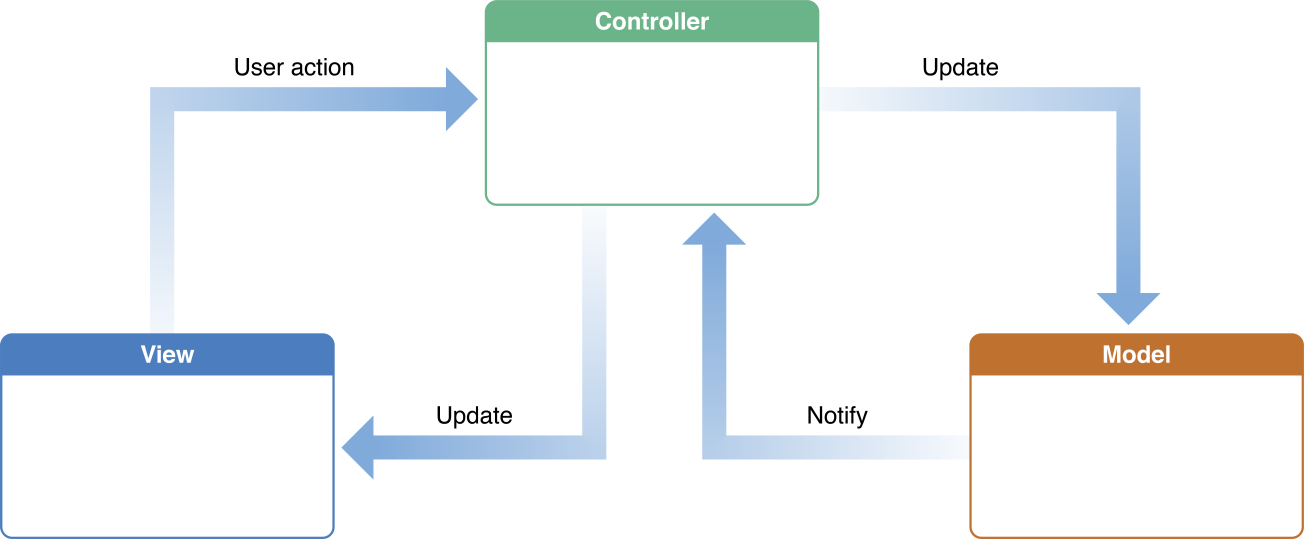
\includegraphics[width=0.99\textwidth]{./pictures/architektury/model_view_controller}
 \caption[Model-View-Controller diagram]{Model-View-Controller diagram \cite{mvc-pic}}\label{fig:mvc}
\end{figure}

\begin{figure}[h]\centering
 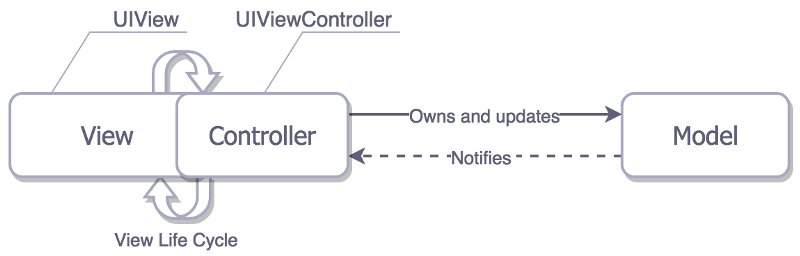
\includegraphics[width=0.99\textwidth]{./pictures/architektury/appleMVC}
 \caption[Model-View-Controller při vývoji iOS aplikace]{Model-View-Controller při vývoji iOS aplikace \cite{mvc-apple-pic}}\label{fig:mvc-apple}
\end{figure}

\subsection{MVVM}
Architektura MVVM má obdobné koncepce jako MVC. Jedná se také o zkratku, tentokrát \uv{Model-View-ViewModel}. \cite{MVVMMicrosoft}
\begin{itemize}
\item $Model$ je totožný s $Model$ vrstvou architektury MVC, jedná se tedy o datovou část aplikace.
\item $View$ prezentuje aplikační data uživateli a monitoruje jeho akce. Však, jak již bylo zmíněno dříve, u iOS aplikací se jedná spíše o vrstvu\\ $View/View controller$. Tato vrstva obsahuje pouze minimum logiky aplikace a reaguje hlavně na $ViewModel$.  \cite{Morrison}
\item $ViewModel$ spojuje $View$ a $Model$ a zajišťuje hlavní logiku aplikace. $ViewModel$ tedy komunikuje s  $Model$ a jeho metodami a následně připravuje data pro $View$. Obsahuje také implementaci funkcí, které reagují a zpracovávají akce uživatele např.: kliknutí na tlačítko. \cite{MVVMMicrosoft}
\end{itemize}

Tedy pro shrnutí rozdílů MVC a MVVM u iOS bych zmínil to, že iOS MVC má ve výsledku téměř jen dvě vrstvy $View/View controller$ a $Model$. Když potom uvažujeme architekturu MVVM ,$View/View controller$  je opravdu pouze jednou vrstvou a mezi ní a $Model$ je vložena nová vrstva  $ViewModel$, která je spojuje, a do které je přesunuta i většina aplikační logiky.

Mezi výhody architektury MVVM oproti MVC patří např.:
\begin{itemize}
\item poskytuje návrhový princip tzv. separation of concerns, neboli oddělení zájmů;
\item zlepšuje možnost testovatelnosti aplikace.
\end{itemize}

\begin{figure}[h]\centering
 \includegraphics[width=0.99\textwidth]{./pictures/architektury/MVVM}
 \caption[Model-View-ViewModel architektura]{Model-View-ViewModel architektura \cite{mvvm-pic}}\label{fig:mvvm}
\end{figure}

\subsection{VIPER}
VIPER je poslední rozebíranou možností, co se týče architektur. I zde je název složen z prvních písmen jednotlivých vrstev architektury, tedy \uv{View, Interactor, Presenter, Entity, Router}.
\begin{itemize}
\item $View$  zobrazuje data uživateli a předává uživatelovi vstupy vrstvě $Presenter$.
\item $Interactor$ obsahuje logiku aplikace spojenou s daty ($Entity$).
\item $Presenter$ vrstva má na starosti $View$ logiku.  Reaguje tedy na uživatelovy akce a komunikuje s vrstvou $Interactor$, od ní také přijímá nová data. \cite{Orlov}
\item $Entity$ jsou datové objekty aplikace přístupné pouze části $Interactor$.
\item $Routing$ obsahuje navigační logiku. \cite{VIPER}
\end{itemize}

Mezi výhody architektury VIPER znovu patří např.:
\begin{itemize}
\item dobře rozděluje odpovědnosti;
\item zlepšuje možnost testovatelnosti aplikace. \cite{Orlov}
\end{itemize}

Tato architektura však může být zbytečně složitá pro menší aplikace. \cite{Orlov}

\begin{figure}[h]\centering
 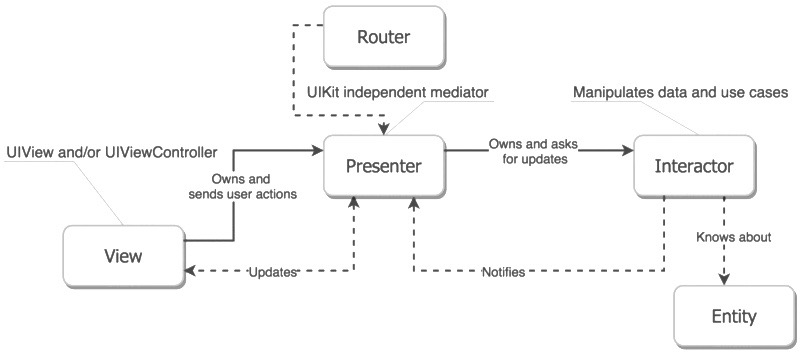
\includegraphics[width=0.99\textwidth]{./pictures/architektury/viper.jpg}
 \caption[VIPER architektura]{VIPER architektura \cite{viper-pic}}\label{fig:viper}
\end{figure}

\section{Funkcionálně reaktivní programování}
Funkcionálně reaktivní programování je kombinací funkcionálního a reaktivního programování, díky němuž dokáže aplikace dynamicky měnit stav a chování v závislosti na událostech přicházejících za nějaký čas. \cite{technopediaFRP}

Pro vysvětlení, co je reaktivní programování cituji \cite{Ztaltz2014} \uv{reaktivní programování je programování s asynchronními datovými toky}.

Na spojení funkcionální a reaktivního programování může dívat i jako na návrhový vzor $observer$. \cite{Blackheath2016} Pozorujeme tedy např. určité vstupní pole, tlačítko nebo i dotaz na server a jsme informování o každé změně v podobě asynchronního datového toku. Na tyto datové toky je možné aplikovat funkcionální programování. Je tedy možné toky spojovat ($merge$), filtrovat ($filter$) pouze události, které nás zajímají,  mapovat ($map$) jeden tok na nový a další. \cite{Ztaltz2014}

\subsection{FRP frameworky pro iOS}
V této kapitole jsou pouze rozebrány základy jednotlivých frameworků, podrobnější vysvětlení (zvoleného frameworku) společně s ukázkami jsou k nalezení v kapitole \nameref{chap:realizace}.
\subsubsection{ReactiveSwift}
ReactiveSwift je prvním frameworkem pro iOS podporující FRP. Obsahuje řadu základních prvků ($Signal$, $SignalProducer$, $Property$, $Action$\ldots) a operátorů podporujících myšlenku \uv{tok hodnot za čas}. \cite{ReactiveSwift}
\subsubsection{ReactiveCocoa}
ReactiveCocoa je další z FRP frameworků pro iOS. ReactiveCocoa rozšiřuje různé aspekty Apple Cocoa frameworku základními prvky frameworku ReactiveSwift. Umožňuje vazbu na prvky uživatelského rozhraní, u interaktivních prvků napojuje $Signal$ a $Action$ pro kontrolu událostí a změn. Dále také umožňuje vytvářet signály na volání metod (např. i pro UIKit třídy). \cite{ReactiveCocoa}
\subsubsection{RxSwift}
RxSwift je Swift verzí knihovny Reactive Extensions (Rx). \cite{RxSwift} Tato knihovna umožňuje vytvářet aplikace založené na událostech a asynchronních datových tocích pomocí tzv. Observables. \cite{RxNET} I přesto, že RxSwift není striktně FRP frameworkem, \cite{ReactiveExtensionsDocs} je zde uváděn, a to z důvodu velkého využití knihovny Reactive Extensions i na jiných platformách např.: JavaScript, C\#, Python. \cite{ReactiveExtensions}

\section{Persistence dat}

\chapter{Realizace}
\label{chap:realizace}

\section{iOS aplikace a Swift}
\section{Unit testy}
\section{Použité nástroje při vývoji}
\section{Uživatelské testování}

\section{Postupy FRP v aplikaci}
\section{Zhodnocení MVVM a FRP}

\begin{conclusion}
	%sem napište závěr Vaší práce
\end{conclusion}

\bibliographystyle{csn690}
\bibliography{mybibliographyfile}

\appendix

\chapter{Seznam použitých zkratek}
% \printglossaries
\begin{description}
	\item[FRP] Funkcionálně reaktivní programování
	\item[MVC] Model View Controller
	\item[MVVM] Model View ViewModel
	\item[VIPER] View Interactor Presenter Entity Router
	\item[PC] Personal Computer
	\item[EASA] European Aviation Safety Agency
	\item[PIC] Pilot-in-command
	\item[SE] Single engine
	\item[ME] Multi engine
	\item[SPIC] Student PIC
	\item[PICUS] PIC under supervision
	\item[FSTD] flight simulation training devices
	\item[FI] Flight instructor
	\item[FE] Flight examiner
	\item[LAPL] Light Aircraft Pilot Licence
	\item[SPL] Sailplane Pilot Licence
	\item[BPL] Balloon Pilot Licence
	\item[PPL] Private Pilot Licence
\end{description}


% % % % % % % % % % % % % % % % % % % % % % % % % % % % 
% % Tuto kapitolu z výsledné práce ODSTRAŇTE.
% % % % % % % % % % % % % % % % % % % % % % % % % % % % 
% 
% \chapter{Návod k~použití této šablony}
% 
% Tento dokument slouží jako základ pro napsání závěrečné práce na Fakultě informačních technologií ČVUT v~Praze.
% 
% \section{Výběr základu}
% 
% Vyberte si šablonu podle druhu práce (bakalářská, diplomová), jazyka (čeština, angličtina) a kódování (ASCII, \mbox{UTF-8}, \mbox{ISO-8859-2} neboli latin2 a nebo \mbox{Windows-1250}). 
% 
% V~české variantě naleznete šablony v~souborech pojmenovaných ve formátu práce\_kódování.tex. Typ může být:
% \begin{description}
% 	\item[BP] bakalářská práce,
% 	\item[DP] diplomová (magisterská) práce.
% \end{description}
% Kódování, ve kterém chcete psát, může být:
% \begin{description}
% 	\item[UTF-8] kódování Unicode,
% 	\item[ISO-8859-2] latin2,
% 	\item[Windows-1250] znaková sada 1250 Windows.
% \end{description}
% V~případě nejistoty ohledně kódování doporučujeme následující postup:
% \begin{enumerate}
% 	\item Otevřete šablony pro kódování UTF-8 v~editoru prostého textu, který chcete pro psaní práce použít -- pokud můžete texty s~diakritikou normálně přečíst, použijte tuto šablonu.
% 	\item V~opačném případě postupujte dále podle toho, jaký operační systém používáte:
% 	\begin{itemize}
% 		\item v~případě Windows použijte šablonu pro kódování \mbox{Windows-1250},
% 		\item jinak zkuste použít šablonu pro kódování \mbox{ISO-8859-2}.
% 	\end{itemize}
% \end{enumerate}
% 
% 
% V~anglické variantě jsou šablony pojmenované podle typu práce, možnosti jsou:
% \begin{description}
% 	\item[bachelors] bakalářská práce,
% 	\item[masters] diplomová (magisterská) práce.
% \end{description}
% 
% \section{Použití šablony}
% 
% Šablona je určena pro zpracování systémem \LaTeXe{}. Text je možné psát v~textovém editoru jako prostý text, lze však také využít specializovaný editor pro \LaTeX{}, např. Kile.
% 
% Pro získání tisknutelného výstupu z~takto vytvořeného souboru použijte příkaz \verb|pdflatex|, kterému předáte cestu k~souboru jako parametr. Vhodný editor pro \LaTeX{} toto udělá za Vás. \verb|pdfcslatex| ani \verb|cslatex| \emph{nebudou} s~těmito šablonami fungovat.
% 
% Více informací o~použití systému \LaTeX{} najdete např. v~\cite{wikilatex}.
% 
% \subsection{Typografie}
% 
% Při psaní dodržujte typografické konvence zvoleného jazyka. České \uv{uvozovky} zapisujte použitím příkazu \verb|\uv|, kterému v~parametru předáte text, jenž má být v~uvozovkách. Anglické otevírací uvozovky se v~\LaTeX{}u zadávají jako dva zpětné apostrofy, uzavírací uvozovky jako dva apostrofy. Často chybně uváděný symbol "{} (palce) nemá s~uvozovkami nic společného.
% 
% Dále je třeba zabránit zalomení řádky mezi některými slovy, v~češtině např. za jednopísmennými předložkami a spojkami (vyjma \uv{a}). To docílíte vložením pružné nezalomitelné mezery -- znakem \texttt{\textasciitilde}. V~tomto případě to není třeba dělat ručně, lze použít program \verb|vlna|.
% 
%Více o~typografii viz \cite{kobltypo}.
% 
% \subsection{Obrázky}
% 
% Pro umožnění vkládání obrázků je vhodné použít balíček \verb|graphicx|, samotné vložení se provede příkazem \verb|\includegraphics|. Takto je možné vkládat obrázky ve formátu PDF, PNG a JPEG jestliže používáte pdf\LaTeX{} nebo ve formátu EPS jestliže používáte \LaTeX{}. Doporučujeme preferovat vektorové obrázky před rastrovými (vyjma fotografií).
% 
% \subsubsection{Získání vhodného formátu}
% 
% Pro získání vektorových formátů PDF nebo EPS z~jiných lze použít některý z~vektorových grafických editorů. Pro převod rastrového obrázku na vektorový lze použít rasterizaci, kterou mnohé editory zvládají (např. Inkscape). Pro konverze lze použít též nástroje pro dávkové zpracování běžně dodávané s~\LaTeX{}em, např. \verb|epstopdf|.
% 
% \subsubsection{Plovoucí prostředí}
% 
% Příkazem \verb|\includegraphics| lze obrázky vkládat přímo, doporučujeme však použít plovoucí prostředí, konkrétně \verb|figure|. Například obrázek \ref{fig:float} byl vložen tímto způsobem. Vůbec přitom nevadí, když je obrázek umístěn jinde, než bylo původně zamýšleno -- je tomu tak hlavně kvůli dodržení typografických konvencí. Namísto vynucování konkrétní pozice obrázku doporučujeme používat odkazování z~textu (dvojice příkazů \verb|\label| a \verb|\ref|).
% 
% \begin{figure}\centering
% 	
\includegraphics[width=0.5\textwidth, angle=30]{cvut-logo-bw}
% 	\caption[Příklad obrázku]{Ukázkový obrázek v~plovoucím prostředí}\label{fig:float}
% \end{figure}
% 
% \subsubsection{Verze obrázků}
% 
% % Gnuplot BW i barevně
% Může se hodit mít více verzí stejného obrázku, např. pro barevný či černobílý tisk a nebo pro prezentaci. S~pomocí některých nástrojů na generování grafiky je to snadné.
% 
% Máte-li například graf vytvořený v programu Gnuplot, můžete jeho černobílou variantu (viz obr. \ref{fig:gnuplot-bw}) vytvořit parametrem \verb|monochrome dashed| příkazu \verb|set term|. Barevnou variantu (viz obr. \ref{fig:gnuplot-col}) vhodnou na prezentace lze vytvořit parametrem \verb|colour solid|.
% 
% \begin{figure}\centering
% 	\includegraphics{gnuplot-bw}
% 	\caption{Černobílá varianta obrázku generovaného programem Gnuplot}\label{fig:gnuplot-bw}
% \end{figure}
% 
% \begin{figure}\centering
% 	\includegraphics{gnuplot-col}
% 	\caption{Barevná varianta obrázku generovaného programem Gnuplot}\label{fig:gnuplot-col}
% \end{figure}
% 
% 
% \subsection{Tabulky}
% 
% Tabulky lze zadávat různě, např. v~prostředí \verb|tabular|, avšak pro jejich vkládání platí to samé, co pro obrázky -- použijte plovoucí prostředí, v~tomto případě \verb|table|. Například tabulka \ref{tab:matematika} byla vložena tímto způsobem.
% 
% \begin{table}\centering
% 	\caption[Příklad tabulky]{Zadávání matematiky}\label{tab:matematika}
% 	\begin{tabular}{|l|l|c|c|}\hline
% 		Typ		& Prostředí		& \LaTeX{}ovská zkratka	& \TeX{}ovská zkratka	\tabularnewline \hline \hline
% 		Text		& \verb|math|		& \verb|\(...\)|	& \verb|$...$|		\tabularnewline \hline
% 		Displayed	& \verb|displaymath|	& \verb|\[...\]|	& \verb|$$...$$|	\tabularnewline \hline
% 	\end{tabular}
% \end{table}
% 
% % % % % % % % % % % % % % % % % % % % % % % % % % % % 

\chapter{Obsah přiloženého CD}

%upravte podle skutecnosti

\begin{figure}
	\dirtree{%
		.1 readme.txt\DTcomment{stručný popis obsahu CD}.
		.1 exe\DTcomment{adresář se spustitelnou formou implementace}.
		.1 src.
		.2 impl\DTcomment{zdrojové kódy implementace}.
		.2 thesis\DTcomment{zdrojová forma práce ve formátu \LaTeX{}}.
		.1 text\DTcomment{text práce}.
		.2 thesis.pdf\DTcomment{text práce ve formátu PDF}.
		.2 thesis.ps\DTcomment{text práce ve formátu PS}.
	}
\end{figure}

\end{document}
